\chapter{SHA-3}

For our project we chose to study BLAKE, Gr{\o}stl and Keccak, out of the 5 finalists, in the SHA-3 competition. 
All the five finalist were found to be secure, devoid of any weakness that can be practically exploited. Keccak
was chosen, since it was the winner of SHA-3 competition, and is the basis for the current SHA-3 in draft.
Keccak has sponge as design basis, BLAKE is based on HAIFA, and Gr{\o}stl
is based on Merkle-Damg\r{a}rd design. The selection of these three, gives an opportunity to observe the effects 
of different design for reduced hash functions. Thus I chose to go with BLAKE and Gr{\o}stl for comparison with
Keccak in this project. Naveen Kandakumar has studied the rebound attacks in JH \cite{00043}, while Darryl
Clyde Eychner did a statiscal analysis on BLAKE and Skein \cite{00030}, which were the other SHA-3 finalists. The
latest Federal information processing standard(FIPS) publication 202, as of May 2014, has standardised SHA-3 to
be a variant of Keccak, where the input message is concatenated with bits related to domain, before processed 
for hashing.

\section{SHA-3}

As per the latest proposed draft, SHA-3 contains 4 cryptographic hash function variations of Keccak for digest sizes
224, 256, 384 and 512; along with two extendable output functions(XOF) \cite{00042}. XOF are hash functions, whose 
output can be extended to desired length.

\begin{table}
  \begin{center}
    \begin{tabular}{ | c | c | c | c | c | } \hline
    \multirow{2}{*}{{\bf Function}} & \multirow{2}{*}{{\bf Output size}} & \multicolumn{3}{ c| }{{\bf Security strength in bits}} \\ \cline{3-5}
                &     & {\bf Collision} & {\bf Preimage}       & {\bf 2nd Preimage} \\ \Xhline{2\arrayrulewidth}
    SHA-1       & 160 & \textless \thickspace80    & 160       & 160 - $L(M)$ \\ \Xhline{2\arrayrulewidth}
    SHA-224     & 224 & 112             & 224                  & min(224, 256 - $L(M)$) \\ \hline
    SHA-512/224 & 224 & 112             & 224                  & 224 \\ \hline
    SHA-256     & 256 & 128             & 256                  & 256 - $L(M)$ \\ \hline
    SHA-512/256 & 256 & 128             & 256                  & 256 \\ \hline
    SHA-384     & 384 & 192             & 384                  & 384 \\ \hline
    SHA-512     & 512 & 256             & 512                  & 512 - $L(M)$ \\ \Xhline{2\arrayrulewidth}
    SHA3-224    & 224 & 112             & 224                  & 224 \\ \hline
    SHA3-256    & 256 & 128             & 256                  & 256 \\ \hline
    SHA3-384    & 384 & 192             & 384                  & 384 \\ \hline
    SHA3-512    & 512 & 256             & 512                  & 512 \\ \Xhline{2\arrayrulewidth}
    SHAKE128    & $d$ & min($d$/2, 128) & $\geq$ min($d$, 128) & min($d$, 128) \\ \hline
    SHAKE256    & $d$ & min($d$/2, 256) & $\geq$ min($d$, 256) & min($d$, 256) \\ \hline
    \end{tabular}
    \caption{Security strength of SHA-1, SHA-2, SHA-3 functions \cite{00042}}
  \end{center}
\end{table}

The Keccak variants are denoted by KECCAK[c] where c is the capacity of the sponge construction used for Keccak
function. The message that is to be hashed is concatenated with two bits, and the output digest length is mentioned
as parameters to the Keccak function for SHA-3.
\begin{center}
SHA3-224(M) = KECCAK[448](M $\vert \vert$ 01, 224) \\
SHA3-256(M) = KECCAK[512](M $\vert \vert$ 01, 256) \\
SHA3-384(M) = KECCAK[768](M $\vert \vert$ 01, 384) \\
SHA3-512(M) = KECCAK[1024](M $\vert \vert$ 01, 512)
\end{center}
The capacity of each of the hash function is twice that of the digest length. The input string is concatenated with two
bits 01, to support domain separation. The XOF are called SHAKE128 and SHAKE256, where the suffix 128 and 256, denote
security strength of the functions. SHAKE nomenclature comes from the combination of words, SHA and Keccak. The XOF
can be defined as 
\begin{center}
SHAKE128(M, d) = KECCAK[256](M $\vert \vert$ 1111, d) \\
SHAKE256(M, d) = KECCAK[512](M $\vert \vert$ 1111, d)
\end{center}
Here the d denotes digest size, since the output size can be varied as per parameter d. There are two capacities available
for SHAKE, that of being 256 and 512, that give the security margin of 128 and 256 respectively. The message before
being provided as input to SHAKE is concatenated  with 4 bits of 1. The first two bits of 1 are for domain separation,
while the rest 2 bits of 1 are for compatibility with Sakura coding, that enables tree hashing, in which parallel
processing can be applied.

\section{Keccak}
Keccak hash function, is built on sponge construction, which can input and output arbitrary length strings. The sponge
construction has two phases. First is absorb, where the input message is ingested in blocks of defined bit rate interleaved
with the permutations. The second phase is squeeze phase, where the blocks of output are squeezed out as per bit rate. 
The Keccak, state is different in the sense that, the permutations work on a 3 dimensional block, cube
structure rather than linear strings, or 2 dimensional arrays.

  \subsection{Keccak state, sponge functions and padding} 
  \begin{figure}[h]
    \begin{center}
      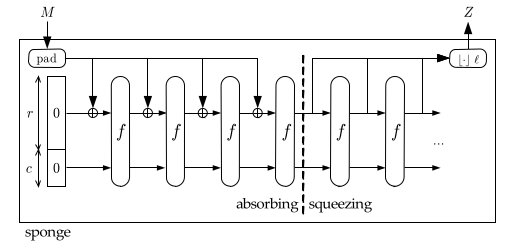
\includegraphics[width=5.5in]{keccakspongeconstruction.jpg}
    \end{center}
    \caption{Sponge construction $Z = Sponge[f, pad, r](M, l)$ \cite{00016}}
    \label{fig:lab}
  \end{figure}

  The sponge construction is used to build function $SPONGE[f, pad, r]$ which inputs and outputs variable length strings 
  \cite{00016}. It uses fixed length permutation $f$, a padding "pad", and parameter bit rate 'r'. The permutations are 
  operated on fixed number of bits, width $b$. The value $c = b - r$ is the capacity of the sponge function. The width 
  $b$ in Keccak defines the state size which can be any of the following \{25, 50, 100, 200, 400, 800, 1600\} number of 
  bits. 
  
  \begin{figure}
    \begin{center}
      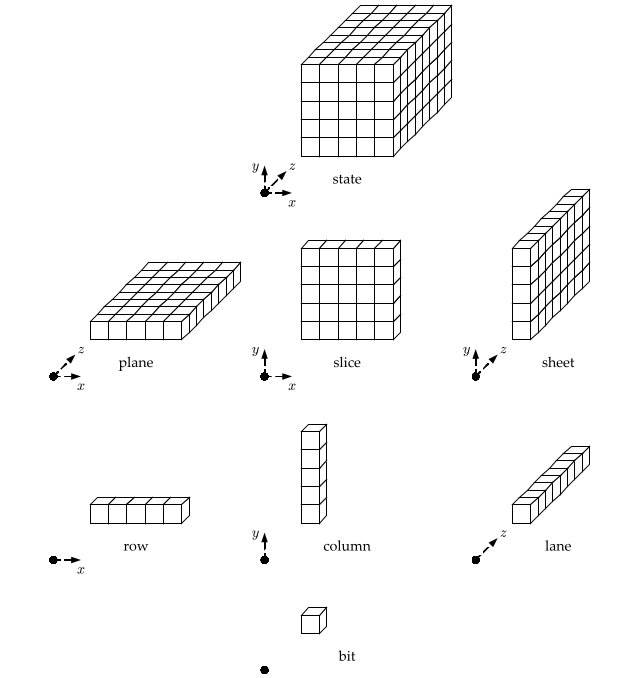
\includegraphics[width=6.5in]{keccakstateterminology.jpg}
    \end{center}
    \caption{Sponge construction $Z = Sponge[f, pad, r](M, l)$ \cite{00015}}
    \label{fig:lab}
  \end{figure}

  The state in Keccak can be represented as a cube having bits, as shown in figure 3.9. The initial state to the sponge
  construction has value 'b' number of 0 bits(represented as $0^{b}$), and called the root state. The root state has fixed
  value and should not be considered as initial value to sponge construction. The different number of state produces
  the Keccak family of hash function variations denoted by $KECCAK-f[b]$.
  
  The varying number of states can be visualized as state having varying number or $l$ number of slices. The width $b$ is
  defined as $b = 25 \times 2^{l}$, where $l$ takes values from 0 to 6.
  
  \begin{algorithm}
    \caption{The sponge construction $SPONGE[f, pad, r]$ \cite{00016}}
    \begin{algorithmic}[1]
      \Require $r < b$
      \State {\bf Interface:} Z = sponge($M, l$) with $M \in \mathbb{Z}^{*}_{2}$, integer $ l > 0$ and $Z \in \mathbb{Z}^{l}_{2}$
      \State $P = M \parallel pad[r](\mid M \mid)$
      \State $s = 0^{b}$
      \State \For {$i = 0 \thickspace to \mid P \mid_{r} - 1$}
        \State $s = s \oplus ( P_{i} \parallel 0^{b - r})$
        \State $s = f(s)$
      \State \EndFor
      \State $ Z = \lfloor s \rfloor_{r}$
      \State \While $\mid Z \mid_{r} r < l $
        \State $s = f(s)$
        \State $Z = Z \parallel \lfloor s \rfloor_{r}$
      \State \EndWhile
      \State \Return $\lfloor Z \rfloor_{l}$ 
    \end{algorithmic}
  \end{algorithm}

  Algorithm 3.2 shows how the sponge construction applied to $KECCAK-f[r + c]$, with multi-rate padding, length of a 
  string $M$ is denoted by $\mid M \mid $. The string $M$ can also be considered as having blocks of size say x,
  and those number of blocks are shown as $\mid M \mid_{x}$. The $\lfloor M \rfloor_{l}$ denotes the string
  $M$ truncated to its first $l$ bits.
  
  The multi-rate padding in Keccak is denoted as $pad \thickspace 1 0^{*}1$ , where a bit '1' is appended to message, 
  followed by minimum number of zeros, and a single bit 1, so that resultant block is multiple of block length $b$.
  \begin{center}$KECCAK[r, c] \doteq SPONGE[KECCAK-f[r + c], pad1 0^{*}1, r]$ \end{center}
  Where $ r > 0$ and $r + c$ is the width. The default value of $r$ is $1600 - c$, and the default value of $c$ is 576.
  \begin{center}$KECCAK[c] \doteq KECCAK[r = 1600 - c, c],$\end{center}
  \begin{center}$KECCAK[] \doteq KECCAK[c = 576]$\end{center}
    
  \subsection{Permutations}

  The $KECCAK-f[b]$ permutations are operated on state represented as a[5][5][w], with w = $2^{l}$, where l can be any value
  from 0 to 6. The position in this 3 dimensional state is given by $a[x][y][z]$ where $x, y \in \mathbb{Z}_{5}$ and $z \in 
  \mathbb{Z}_{w}$. The mapping of the bits from the input message 's' to state 'a' is like this $s[w (5y + x) + z] = a[x][y][z]$.
  The $x, y$ coordinates are taken modulo 5, while the $z$ coordinate is taken as modulo $w$ \cite{00015}.

  There are five steps, for a permutation round R. 
  \begin{center}$R = \iota \circ \chi \circ \pi \circ \rho \circ \theta$\end{center}
  The permutations are repeated for $12 + 2l$ times, with $l$ dependent on the variant chosen. \\
  \begin{align*}
    \theta &: a[x][y][z] & \gets & \thickspace a[x][y][z] + \displaystyle\sum\limits_{y' = 0}^{4} a[x - 1][y'][z] + \displaystyle\sum\limits_{y' = 0}^{4} a[x + 1][y'][z - 1], \\
    \rho &: a[x][y][z] & \gets & \thickspace a[x][y][z - (t + 1)(t + 2) / 2], \\
    & & & \thickspace t \thickspace satisfying \thickspace 0 \leq t < 24 \thickspace and \thickspace
    \begin{pmatrix} 0 & 1 \\ 2 & 3 \end{pmatrix}^{t} \begin{pmatrix} 1 \\ 0 \end{pmatrix} = \begin{pmatrix} x \\ y \end{pmatrix}
    in \thickspace GF(5)^{2 \times 2}, \\
    & & & \thickspace or \thickspace t = -1 \thickspace if \thickspace x = y = 0, \\
    \pi &: a[x][y] & \gets & \thickspace a[x'][y'], \thickspace with \thickspace
    \begin{pmatrix} x \\ y \end{pmatrix} = \begin{pmatrix} 0 & 1 \\ 2 & 3 \end{pmatrix} \begin{pmatrix} x' \\ y'\end{pmatrix}, \\
    \chi &: a[x] & \gets & \thickspace a[x] + (a[x + 1] + 1) \thickspace a[x + 2], \\
    \iota &: a & \gets & \thickspace a + RC[i_{r}].
  \end{align*}

  The addition and the multiplications are in Galois field GF(2), except for the round constants $RC[i_{r}]$. The round constants 
  are given by
  \begin{center}$RC[i_{r}][0][0][2^{j} - 1] = rc[j + 7i_{r}]$ for all $ 0 \leq j \leq l$,\end{center}
  and the rest are zeros. The value of $rc[t] \in GF(2)$ is output of linear feedback shift register given as
  \begin{center}$rc[t] = (x^{t} \thickspace mod \thickspace x^{8} + x^{6} + x^{5} + x^{4} + 1)$ mod x in GF(2)[$x$].\end{center}

  \begin{figure}
    \begin{center}
      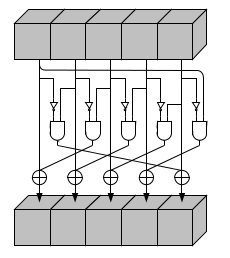
\includegraphics[width=2.3in]{keccakchi.jpg}
    \end{center}
    \caption{$\chi$ applied to a single row \cite{00015}.}
    \label{fig:lab}
  \end{figure}

  \begin{algorithm}
    \caption{ $\chi$ transformation KECCAK \cite{00015}.}
    \begin{algorithmic}[1]
      \State \For {$y = 0 \thickspace to \thickspace 4$}
      \State \For {$x = 0 \thickspace to \thickspace 4$}
      $A[x, y] = a[x, y] \oplus ((NOT \thickspace a[x + 1, y]) \thickspace AND \thickspace a[x + 2, y])$
      \State \EndFor
      \State \EndFor
    \end{algorithmic}
  \end{algorithm}
  
  \begin{figure}
    \begin{center}
      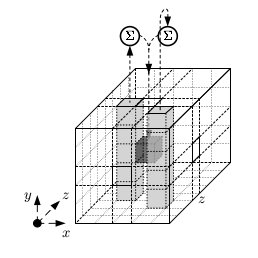
\includegraphics[width=2.7in]{keccaktheta.jpg}
    \end{center}
    \caption{$\theta$ applied to a single bit \cite{00015}.}
    \label{fig:lab}
  \end{figure}

  \begin{algorithm}
    \caption{ $\theta$ transformation KECCAK \cite{00015}.}
    \begin{algorithmic}[1]
      \State \For {$x = 0 \thickspace to \thickspace 4$}
      \State $C[x] = a[x, 0]$
      \State \For {$y = 1 \thickspace to \thickspace 4$}
      $C[x] = C[x] \oplus a[x, y]$
      \State \EndFor
      \State \EndFor
      \State \For {$x = 0 \thickspace to \thickspace 4$}
      \State $D[x] = C[x - 1] \oplus ROT(C[x + 1], 1)$
      \State \For {$y = 0 \thickspace to \thickspace 4$}
      \State $A[x, y] = a[x, y] \oplus D[x]$
      \State \EndFor
      \State \EndFor
    \end{algorithmic}
  \end{algorithm}

  \begin{algorithm}
    \caption{ $\pi$ transformation KECCAK \cite{00015}.}
    \begin{algorithmic}[1]
      \State \For {$x = 0 \thickspace to \thickspace 4$}
      \State \For {$y = 1 \thickspace to \thickspace 4$}
      \State $\begin{pmatrix} X \\ Y \end{pmatrix} = \begin{pmatrix} 0 & 1 \\ 2 & 3 \end{pmatrix} \begin{pmatrix}x \\ y \end{pmatrix}$
      \State $A[X, Y] = a[x, y]$
      \State \EndFor
      \State \EndFor
    \end{algorithmic}
  \end{algorithm}

  \begin{figure}
    \begin{center}
      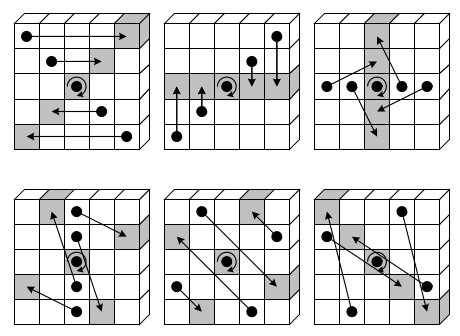
\includegraphics[width=4.75in]{keccakpi.jpg}
    \end{center}
    \caption{$\pi$ applied to a single slice \cite{00015}}
    \label{fig:lab}
  \end{figure}

  \begin{algorithm}
    \caption{ $\rho$ transformation KECCAK \cite{00015}}
    \begin{algorithmic}[1]
      \State $A[0, 0] = a[0, 0]$
      \State $\begin{pmatrix} x \\ y \end{pmatrix} = \begin{pmatrix} 1 \\ 0 \end{pmatrix}$
      \State \For{$t = 0 \thickspace to \thickspace 23$}
      \State $A[x, y] = ROT(a[x, y], (t + 1)(t + 2) / 2)$
      \State $\begin{pmatrix} x \\ y \end{pmatrix} = \begin{pmatrix} 0 & 1 \\ 2 & 3 \end{pmatrix} \begin{pmatrix}x \\ y \end{pmatrix}$
      \State \EndFor
    \end{algorithmic}
  \end{algorithm}

  \begin{figure}
    \begin{center}
      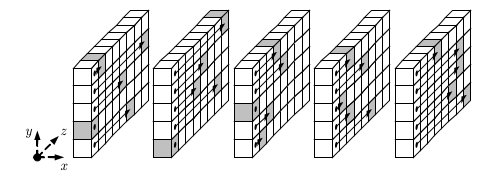
\includegraphics[width=5.1in]{keccakrho.jpg}
    \end{center}
    \caption{$\rho$ transformation applied to lanes \cite{00015}}
    \label{fig:lab}
  \end{figure}

  \begin{table}
    \begin{center}
      \begin{tabular}{ c | *{5}{c}}
                & $x = 2$ & $x = 4$ & $x = 0$ & $x = 1$ & $x = 2$ \\ \hline
        $y = 2$ & 153     & 231     & 3       & 10      & 171     \\
        $y = 1$ & 55      & 276     & 36      & 300     & 6       \\
        $y = 0$ & 28      & 91      & 0       & 1       & 190     \\
        $y = 4$ & 120     & 78      & 210     & 66      & 253     \\
        $y = 3$ & 21      & 136     & 105     & 45      & 15      \\
      \end{tabular}
      \caption{Offsets for $\rho$ transformation \cite{00015}}
    \end{center}
  \end{table}
  
\section{BLAKE} 

BLAKE \cite{00002} hash function is built on HAIFA (HAsh Iterative FrAmework) structure \cite{00020} which is an improved
version of Merkle-Damg\r{a}rd design. It provides resistance to long-message, second pre-image attack and provides a 
salting option, that BLAKE uses \cite{00021}.
The design is local wide-pipe which avoids internal collisions. The compression function in BLAKE is tweaked version of 
ChaCha, a stream cipher. 

\begin{table}[h]
  \begin{center}
    \begin{tabular}{ *{6}{c} } \hline
      Algorithm & Word & Message     & Block & Digest & Salt \\ \hline
      BLAKE-224 & 32   & $< 2^{64}$  & 512   & 224    & 128  \\
      BLAKE-256 & 32   & $< 2^{64}$  & 512   & 256    & 128  \\
      BLAKE-384 & 64   & $< 2^{128}$ & 1024  & 384    & 256  \\
      BLAKE-512 & 64   & $< 2^{128}$ & 1024  & 512    & 256  \\ \hline
    \end{tabular}
    \caption{Specification of available input, output, block and salt sizes for various BLAKE hash functions \cite{00002}.}
  \end{center}
\end{table}

\begin{figure}[h]
  \begin{center}
    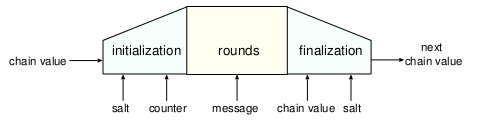
\includegraphics[width=4.75in]{blakelocalwidepipeconstruction.jpg}
  \end{center}
  \caption{Local wide construction of BLAKE's compression function \cite{00002}}
  \label{fig:lab}
\end{figure}

BLAKE has 4 variations of the algorithm shown in table 3.3. Figure 3.7 shows how the individual message blocks are
consumed. The construction takes in 4 inputs, a message; salt, that makes hash function parameter specific; a
counter, which is count of all the bits hashed till then; and lastly a chaining value which is input of the previous 
operation or initial value in case of hash initiation. The compression function is composed of a 4 $\times$ 4 matrix 
of words, where a word is equal to 32 bits for BLAKE-256 variant, while 64 bit for variant BLAKE-512.

\begin{table}[h]
  \begin{center}
    \begin{tabular}{ c l } \hline
      Symbol                  & Meaning \\ \hline
      $\gets$                 & variable assignment \\
      $+$                     & addition modulo $2^{32}$ or (modulo $2^{64}$) \\
      $\ggg k$                & rotate k bits to least significant bits \\
      $\lll k$                 & rotate k bits to most significant bits \\
      $\langle l \rangle_{k}$ & encoding of integer $l$ over $k$ bits \\ \hline
    \end{tabular}
    \caption{Convention of symbols used in BLAKE algorithm}
  \end{center}
\end{table}

\newpage

\subsection{ BLAKE-256 }

The compression function takes following as input
\begin{itemize}
  \item a chaining value of $h = h_{0},\dots, h_{7}$
  \item a message block $m = m_{0},\dots, m_{15}$
  \item a salt $s = s_{0},\dots, s_{3}$
  \item a counter $t = t_{0}, t_{1}$
\end{itemize}
These four inputs of 30 words or 120 bytes, are processed as $h' = compress(h, m, s, t)$ to provide a new
chain value of 8 words.

  \subsubsection{Compression function}

  \begin{itemize}
    \item {\bf Constants}
      
      \begin{table}[H]
        \begin{align*}
             {\tt c_{0}}  &= {\tt 243F6A88} & {\tt c_{1}}  &= {\tt 85A308D3} & {\tt c_{2}}  &= {\tt 13198A2E} & {\tt c_{3}}  &= {\tt 03707344}
          \\ {\tt c_{4}}  &= {\tt A4093822} & {\tt c_{5}}  &= {\tt 299F31D0} & {\tt c_{6}}  &= {\tt 082EFA98} & {\tt c_{7}}  &= {\tt EC4E6C89} 
          \\ {\tt c_{8}}  &= {\tt 452821E6} & {\tt c_{9}}  &= {\tt 38D01377} & {\tt c_{10}} &= {\tt BE5466CF} & {\tt c_{11}} &= {\tt 34E90C6C} 
          \\ {\tt c_{12}} &= {\tt C0AC29B7} & {\tt c_{13}} &= {\tt C97C50DD} & {\tt c_{14}} &= {\tt B5470917} & {\tt c_{15}} &= {\tt 3F84D5B5} 
        \end{align*}
        \caption{16 constants used for BLAKE-256 \cite{00002}}
      \end{table}

      \begin{table}
        \begin{center}
          \begin{tabular}{ c| *{16}{c}} \hline
            $\sigma_{0}$ & 0  & 1  & 2  & 3  & 4  & 5  & 6  & 7  & 8  & 9  & 10 & 11 & 12 & 13 & 14 & 15 \\
            $\sigma_{1}$ & 14 & 10 & 4  & 8  & 9  & 15 & 13 & 6  & 1  & 12 & 0  & 2  & 11 & 7  & 5  & 3  \\
            $\sigma_{2}$ & 11 & 8  & 12 & 0  & 5  & 2  & 15 & 13 & 10 & 14 & 3  & 6  & 7  & 1  & 9  & 4  \\
            $\sigma_{3}$ & 7  & 9  & 3  & 1  & 13 & 12 & 11 & 14 & 2  & 6  & 5  & 10 & 4  & 0  & 15 & 8  \\
            $\sigma_{4}$ & 9  & 0  & 5  & 7  & 2  & 4  & 10 & 15 & 14 & 1  & 11 & 12 & 6  & 8  & 3  & 13 \\
            $\sigma_{5}$ & 2  & 12 & 6  & 10 & 0  & 11 & 8  & 3  & 4  & 13 & 7  & 5  & 15 & 14 & 1  & 9  \\
            $\sigma_{6}$ & 12 & 5  & 1  & 15 & 14 & 13 & 4  & 10 & 0  & 7  & 6  & 3  & 9  & 2  & 8  & 11 \\
            $\sigma_{7}$ & 13 & 11 & 7  & 14 & 12 & 1  & 3  & 9  & 5  & 0  & 15 & 4  & 8  & 6  & 2  & 10 \\
            $\sigma_{8}$ & 6  & 15 & 14 & 9  & 11 & 3  & 0  & 8  & 12 & 2  & 13 & 7  & 1  & 4  & 10 & 5  \\
            $\sigma_{9}$ & 10 & 2  & 8  & 4  & 7  & 6  & 1  & 5  & 15 & 11 & 9  & 14 & 3  & 12 & 13 & 0  \\ \hline
          \end{tabular}
          \caption{Round permutations to be used \cite{00002}}
        \end{center}
      \end{table}
    
    \item {\bf Initialization: } The constants mentioned are used with the salts, and counter along with initial
    value used as chaining input, to create a initial matrix of 4 $\times$ 4, 16 word state.

      \begin{table}[h]
        \begin{center}
          \begin{tabular}{ *{4}{c}}
            $IV_{0}$ = 6A09E667 & $IV_{1}$ = BB67AE85 & $IV_{2}$ = 3C6EF372 & $IV_{3}$ = A54FF53A \\
            $IV_{4}$ = 510E527F & $IV_{5}$ = 9B05688C & $IV_{6}$ = 1F83D9AB & $IV_{7}$ = 5BE0CD19 \\
          \end{tabular}
          \caption{Initial values which become the chaining value for the first message block \cite{00002}}
        \end{center}
      \end{table}
      
    \begin{center}
    $\begin{pmatrix} v_{0} & v_{1} & v_{2} & v_{3} \\ v_{4} & v_{5} & v_{6} & v_{7} \\
                     v_{8} & v_{9} & v_{10} & v_{11} \\ v_{12} & v_{13} & v_{14} & v_{15}\end{pmatrix} 
    \gets
    \begin{pmatrix} h_{0} & h_{1} & h_{2} & h_{3} \\ h_{4} & h_{5} & h_{6} & h_{7} \\
       s_{0} \oplus c_{0} & s_{1} \oplus c_{1} & s_{2} \oplus c_{2} & s_{3} \oplus c_{3} \\ 
       t_{0} \oplus c_{4} & t_{0} \oplus c_{5} & t_{1} \oplus c_{6} & t_{1} \oplus c_{7} \end{pmatrix}$
    \end{center}

    \item {\bf Round function:} After initialisation, the state is subjected to column and diagonal operations, 14
    times. A round operation G acts as per following

    \begin{table}[h]
      \begin{center}
        \begin{tabular}{ *{4}{c}}
        $ G_{0}(v_{0}, v_{8}, v_{12})$ & $G_{1}(v_{1}, v_{5}, v_{9}, v_{13})$ & $G_{2}(v_{2}, v_{6}, v_{10}, v_{14})$ & $G_{3}(v_{3}, v_{7}, v_{11}, v_{15}) $\\
 $G_{4}(v_{0}, v_{5}, v_{10}, v_{15})$ & $G_{5}(v_{1}, v_{6}, v_{11}, v_{12})$ & $G_{6}(v_{2}, v_{7}, v_{8}, v_{13})$ & $G_{7}(v_{3}, v_{4}, v_{9}, v_{14})$
        \end{tabular}
      \end{center}
    \end{table}

    %$ G_{0}(v_{0}, v_{8}, v_{12}) \; G_{1}(v_{1}, v_{5}, v_{9}, v_{13}) \; G_{2}(v_{2}, v_{6}, v_{10}, v_{14}) \; G_{3}(v_{3}, v_{7}, v_{11}, v_{15}) \\
    %G_{4}(v_{0}, v_{5}, v_{10}, v_{15}) \; G_{5}(v_{1}, v_{6}, v_{11}, v_{12}) \; G_{6}(v_{2}, v_{7}, v_{8}, v_{13}) \; G_{7}(v_{3}, v_{4}, v_{9}, v_{14})$

    where the round function $G_{i}(a, b, c, d)$ sets
    
    $
    a \gets a + b + (m_{\sigma_{r}(2i)} \oplus c_{\sigma_{r}(2i + 1)}) \\
    d \gets (d \oplus a) \ggg 16 \\
    c \gets c + d \\
    b \gets (b \oplus c) \ggg 12 \\
    a \gets a + b + (m_{\sigma_{r}(2i + 1)} \oplus c_{\sigma_{r}(2i)}) \\
    d \gets (d \oplus a) \ggg 8 \\
    c \gets c + d \\
    b \gets (b \oplus c) \ggg 7
    $

    The implementation of the G function is shown below.
    \begin{figure}[h]
      \begin{center}
        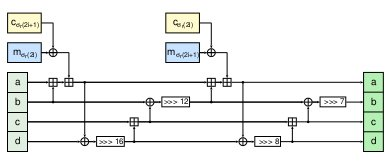
\includegraphics[width=4in]{blakeGfunction.jpg}
      \end{center}
      \caption{The $G_{i}$ function in BLAKE \cite{00002}}
      \label{fig:lab}
    \end{figure}

    \item {\bf Finalization:} The chaining values for the next stage are obtained by XOR of the words from the state 
    matrix, the salt and the initial value.

    $
    h'_{0} \gets h_{0} \oplus s_{0} \oplus v_{0} \oplus v_{8} \\
    h'_{1} \gets h_{1} \oplus s_{1} \oplus v_{1} \oplus v_{9} \\
    h'_{2} \gets h_{2} \oplus s_{2} \oplus v_{2} \oplus v_{10} \\
    h'_{3} \gets h_{3} \oplus s_{3} \oplus v_{3} \oplus v_{11} \\
    h'_{4} \gets h_{4} \oplus s_{0} \oplus v_{4} \oplus v_{12} \\
    h'_{5} \gets h_{5} \oplus s_{1} \oplus v_{5} \oplus v_{13} \\
    h'_{6} \gets h_{6} \oplus s_{2} \oplus v_{6} \oplus v_{14} \\
    h'_{7} \gets h_{7} \oplus s_{3} \oplus v_{7} \oplus v_{15} \\
    $
  \end{itemize}

  \subsubsection{Hashing the message}

  A given input message is padded with a bit '1' followed followed by at most 511 bits of zeros, so that the message 
  size is equal to 447 modulo 512. This padding is followed by a bit '1' and a 64-bit unsigned big-endian representation
  of block length $l$. The padding to a message, can be represented as $m \gets m \parallel 1000 \dots 0001\langle l \rangle_{64}$

  \begin{algorithm}
  \caption{BLAKE Compression procedure \cite{00002}}
  \begin{algorithmic}[1]
    \State $ h^{0} \gets IV $
    \For {$i = 0,\dots, N - 1$}
      \State $h^{i+1} \gets compress(h^{i}, m^{i}, s, l^{i})$
    \EndFor
    \State\Return{$h^{N}$}
  \end{algorithmic}
  \end{algorithm}

  As shown in algorithm 3.1, the BLAKE compression function ingests the padded message block by block, in a loop 
  starting from the initial value, and then sends the last chained value obtained from the finalization to the 
  $\Omega$ truncation function, to obtain the hash value.

\subsection{BLAKE-512}

BLAKE-512 operates on 64-bit words and returns a 64-byte hash value. The chaining value is 512 bit long, message blocks are
1024 bits, salt is 256 bits, and counter size is 128 bits. The difference from BLAKE-256 are in initial values and constants
(tables 3.8 and 3.9) used. Compression function and padding is also tweaked to better suit 64 bit word.

  \begin{table}[H]
    \begin{align*}
      {\tt IV_{0}} &= {\tt 6A09E667F3BCC908} & {\tt IV_{1}} &= {\tt BB67AE8584CAA73B} & {\tt IV_{2}} &= {\tt 3C6EF372FE94F82B} \\
      {\tt IV_{3}} &= {\tt A54FF53A5F1D36F1} & {\tt IV_{4}} &= {\tt 510E527FADE682D1} & {\tt IV_{5}} &= {\tt 9B05688C2B3E6C1F} \\
      {\tt IV_{6}} &= {\tt 1F83D9ABFB41BD6B} & {\tt IV_{7}} &= {\tt 5BE0CD19137E2179} &                                        \\      
    \end{align*}
    \caption{Initial values used for BLAKE-512 \cite{00002}}
  \end{table}
  
  \begin{table}
    \begin{align*}
         {\tt c_{0}}  &= {\tt 243F6A8885A308D3} & {\tt c_{1}}  &= {\tt 13198A2E03707344} & {\tt c_{2}}  &= {\tt A4093822299F31D0} 
      \\ {\tt c_{3}}  &= {\tt 082EFA98EC4E6C89} & {\tt c_{4}}  &= {\tt 452821E638D01377} & {\tt c_{5}}  &= {\tt BE5466CF34E90C6C} 
      \\ {\tt c_{6}}  &= {\tt C0AC29B7C97C50DD} & {\tt c_{7}}  &= {\tt 3F84D5B5B5470917} & {\tt c_{8}}  &= {\tt 9216D5D98979FB1B} 
      \\ {\tt c_{9}}  &= {\tt D1310BA698DFB5AC} & {\tt c_{10}} &= {\tt 2FFD72DBD01ADFB7} & {\tt c_{11}} &= {\tt B8E1AFED6A267E96} 
      \\ {\tt c_{12}} &= {\tt BA7C9045F12C7F99} & {\tt c_{13}} &= {\tt 24A19947B3916CF7} & {\tt c_{14}} &= {\tt 0801F2E2858EFC16} 
      \\ {\tt c_{15}} &= {\tt 636920D871574E69} &                                        &      
    \end{align*}
    \caption{16 constants used for BLAKE-512 \cite{00002}}
  \end{table}
  
  Compression function in BLAKE-512 gets 16 iterations instead of 14 as in BLAKE-256, the rotations are updated and 
  word size increased from 32 bits to 64 bits. $G_{i}(a, b, c, d)$ is given as \\
  $
  a \gets a + b + (m_{\sigma_{r}(2i)} \oplus c_{\sigma_{r}(2i + 1)}) \\
  d \gets (d \oplus a) \ggg 32 \\
  c \gets c + d \\
  b \gets (b \oplus c) \ggg 25 \\
  a \gets a + b + (m_{\sigma_{r}(2i + 1)} \oplus c_{\sigma_{r}(2i)}) \\
  d \gets (d \oplus a) \ggg 16 \\
  c \gets c + d \\
  b \gets (b \oplus c) \ggg 11
  $
  
  Once more than 9 rounds are done, then permutations to be applied from table are selected by modulo 10 of round. 
  For example if round r \textgreater 9 then permutation used is $\sigma_{r \thickspace mod \thickspace 10}$, say 
  r = 15 then permutation would be $\sigma_{15 \thickspace mod \thickspace 10} = \sigma_{5}$.

  For the padding, the message is first padded with bit 1 and then as many zeros required to make the bit length
  equivalent to 895 modulo 1024. After that another bit of value 1 is appended followed by 128-bits unsigned big-endian
  representation of of message length as $m \gets m \parallel 100 \dots 001 \langle l \rangle_{128}$.

\subsection{BLAKE-224 and BLAKE-384}

  \subsubsection{BLAKE-224}
  BLAKE-224 is similar to BLAKE-256, but differs slightly. It has different initial values, different padding and the
  output bits are truncated to first 224 bits.
  \begin{table}[h]
    \begin{center}
      \begin{tabular}{ *{4}{c}}
        $IV_{0}$ = C1059ED8 & $IV_{1}$ = 367CD507 & $IV_{2}$ = 3070DD17 & $IV_{3}$ = F70E5939 \\
        $IV_{4}$ = FFC00B31 & $IV_{5}$ = 68581511 & $IV_{6}$ = 64F98FA7 & $IV_{7}$ = BEFA4FA4 \\
      \end{tabular}
      \caption{Initial values for BLAKE-224 which are taken from SHA-224 \cite{00002}}
    \end{center}
  \end{table}
  The padding differs from BLAKE-256 in way that the bit preceding the message length is replaced by a 0 bit. Which
  is represented as $m \gets m \parallel 100 \dots 000 \langle l \rangle_{64}$.

  \subsubsection{BLAKE-384}
  In BLAKE-384 the output of BLAKE-512 is truncated to 384 bits. The padding differs from BLAKE-512, in way that bit
  preceding the length encoding is 0 and not 1. It can be shown as $m \gets m \parallel 100 \dots 000 \langle l \rangle_{128}$. The
  initial chaining values are given in table 3.11.
  \begin{table}[h]
    \begin{align*}
      {\tt IV_{0}} &= {\tt CBBB9D5DC1059ED8} & {\tt IV_{1}} &= {\tt 629A292A367CD507} & {\tt IV_{2}} &= {\tt 9159015A3070DD17} \\
      {\tt IV_{3}} &= {\tt 152FECD8F70E5939} & {\tt IV_{4}} &= {\tt 67332667FFC00B31} & {\tt IV_{5}} &= {\tt 8EB44A8768581511} \\
      {\tt IV_{6}} &= {\tt DB0C2E0D64F98FA7} & {\tt IV_{7}} &= {\tt 47B5481DBEFA4FA4} &                                        \\      
    \end{align*}
    \caption{Initial values for BLAKE-384 \cite{00002}}
  \end{table}

\newpage

\section{Gr{\o}stl}

Gr{\o}stl is collection of hash functions which produce digest size, ranging from 1 to 64 bytes. The variant of
Gr{\o}stl that returns a message digest of size n, is called Gr{\o}stl-n.

Gr{\o}stl is an iterated hash function, with two two compression functions named P and Q, based on wide trail design
and having distinct permutations. Gr{\o}stl has a byte oriented SP network, and its diffusion layers and S-box 
are identical to AES. The design is a wide-pipe construction, where the internal state size is larger than output 
size, thus preventing most of the generic attacks. None of the permutations are indexed by a key, to prevent attacks
from a weak key schedule \cite{00019}.

  \subsection{The hash function construction}

  The input is padded and then split into l-bit message blocks $m_{1}$,$\ldots$, $m_{t}$, and each message block is
  processed sequentially. The initial $l$-bit chaining value $h_{0}$ = iv is defined, and the blocks $m_{i}$ are
  processed as 

  \begin{center}$ h_{i}\gets f(h_{i-1}, m_{i})\thickspace for \thickspace i = 1,\ldots, t.$\end{center}

  Thus $f$ consumes two $l-bits$ input, and maps to output of $l-bits$. For variants up to 256 bits output, size of $l$ is
  512 bits. And for digest sizes larger than 256 bits, $l$ is 1024 bits.

  \begin{figure}[h]
    \begin{center}
      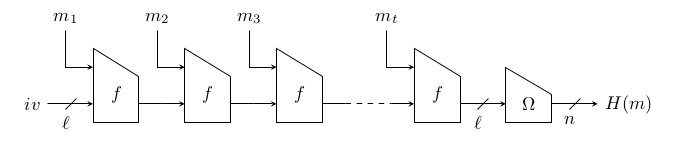
\includegraphics[width=5.5in]{groestlhashfunction.jpg}
    \end{center}
    \caption{Gr{\o}stl hash function \cite{00019}}
    \label{fig:lab}
  \end{figure}

  After the last message block is processed, the last chaining value output is sent through a $\Omega$ function, to get
  the hash output H(M). Figure 3.9 displays the process.
  \begin{center}$H(M) = \Omega(h_{t}),$\end{center}
  The permutation function $f$, is composed of two $l$-bit permutations called P and Q.
  \begin{center}$f(h, m) = P(h \oplus m) \oplus Q(m) \oplus h.$\end{center}
  
  \begin{figure}
    \begin{center}
      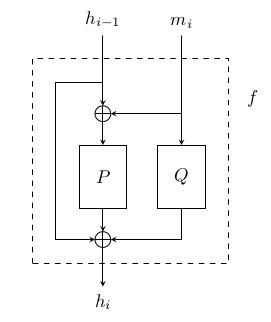
\includegraphics[width=2.5in]{groestlPQfunction.jpg}
    \end{center}
    \caption{Compression functions, where P and Q are $l-bit$ permutations \cite{00019}}
    \label{fig:lab}
  \end{figure}

  The $\Omega$ function consists of a $trunc_{n}(x)$ that outputs only the trailing n bits of input x.
  \begin{center}$\Omega(x) = trunc_{n}( P(x) \oplus x ).$\end{center}

  \begin{figure}
    \begin{center}
      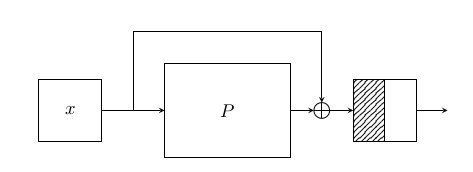
\includegraphics[width=4.5in]{groestlomegafunction.jpg}
    \end{center}
    \caption{Omega truncation function \cite{00019}}
    \label{fig:lab}
  \end{figure}

  In order to fit the varying input length message to the block sizes of $ l $, the message is padded to make it a
  multiple of block size $l$. First bit '1' is
  appended, then\\ $ w = -N - 65 \thickspace mod \thickspace l $, 0 bits are appended; where N is the length of the
  original message. Finally a 64 bit representation of $(N + w + 65) / l $ is padded. Given the need for message length
  to be present in the padding, the maximum size of message digest in bits for Gr{\o}stl-512 version is 
  $2^{73}-577$ bits, and that for 1024 version is $2^{74}-1089$bits.

  \subsection{Design of P and Q permutations}

  There are two variations for P and Q permutations, one each for the digest size lower and higher than 256 bits. P
  and Q, make a round R, that has 4 transformations
  \begin{center}$ R = MixBytes \circ ShiftBytes \circ SubBytes \circ AddRoundConstant $ \end{center}
  The transformations $SubBytes$ and $MixBytes$ are same for all transformation while, $ShiftBytes$ and $AddRoundConstant$
  differ for each of the transformations. The transformations operate on matrix of bytes, with the permutation of lower size
  digest having matrix of 8 rows and 8 columns, while that for larger variant is of 16 columns and 8 rows. The number of 
  rounds for each R is given as recommendation in table 3.12 and the initial values are given in table 3.13.
  
  \begin{table}
    \begin{center}
      \begin{tabular}{ *{3}{c} } \hline
        Permutations            & Digest size & Recommended value of r \\ \hline
        $P_{512}$ and $Q_{512}$   & 8 - 256     & 10 \\
        $P_{1024}$ and $Q_{1024}$ & 264 - 512   & 14 \\ \hline 
      \end{tabular}
      \caption{Recommended number of rounds \cite{00019}}
    \end{center}
  \end{table}

  \begin{table}
    \begin{center}
      \begin{tabular}{ *{2}{c} } \hline
        n   & $iv_{n}$         \\ \hline
        224 & 00 $\dots$ 00 00 e0 \\
        256 & 00 $\dots$ 00 01 00 \\
        384 & 00 $\dots$ 00 01 80 \\
        512 & 00 $\dots$ 00 02 00 \\ \hline
      \end{tabular}
    \caption{Initial values for Gr{\o}stl-n function. The numbers on left denote digest size in bits \cite{00019}.}
    \end{center}
  \end{table}

\newpage
    \subsubsection{Mapping:} of a 64-byte input sequence of 0x00 0x01 0x02 $\ldots$ 3f to a 8 $\times$ 8 matrix is shown 
    in the following matrix. For a 8 $\times$ 16 matrix, the mapping is extended the same way. Mapping the intermediate 
    state values to byte sequence is reverse of this process. \\
     \begin{center}$\mathsf{Input\thickspace Mapping} = \renewcommand\arraystretch{0.75}
      \begin{bmatrix}
        \mathsf{00} & \mathsf{08} & \mathsf{10} & \mathsf{18} & \mathsf{20} & \mathsf{28} & \mathsf{30} & \mathsf{38} \\
        \mathsf{01} & \mathsf{09} & \mathsf{11} & \mathsf{19} & \mathsf{21} & \mathsf{29} & \mathsf{31} & \mathsf{39} \\
        \mathsf{02} & \mathsf{0a} & \mathsf{12} & \mathsf{1a} & \mathsf{22} & \mathsf{2a} & \mathsf{32} & \mathsf{3a} \\
        \mathsf{03} & \mathsf{0b} & \mathsf{13} & \mathsf{1b} & \mathsf{23} & \mathsf{2b} & \mathsf{33} & \mathsf{3b} \\
        \mathsf{04} & \mathsf{0c} & \mathsf{14} & \mathsf{1c} & \mathsf{24} & \mathsf{2c} & \mathsf{34} & \mathsf{3c} \\
        \mathsf{05} & \mathsf{0d} & \mathsf{15} & \mathsf{1d} & \mathsf{25} & \mathsf{2d} & \mathsf{35} & \mathsf{3d} \\
        \mathsf{06} & \mathsf{0e} & \mathsf{16} & \mathsf{1e} & \mathsf{26} & \mathsf{2e} & \mathsf{36} & \mathsf{3e} \\
        \mathsf{07} & \mathsf{0f} & \mathsf{17} & \mathsf{1f} & \mathsf{27} & \mathsf{2f} & \mathsf{37} & \mathsf{3f}
      \end{bmatrix}$\end{center}
      
    \subsubsection{AddRoundConstant:} XORs a round dependant constant to the state matrix say A. It is represented as 
    $A \gets A \oplus C[i]$, where $C[i]$ is the round constant in round $i$. The constants for both P and Q for both
    variations are shown below. $i$ is the round number represented as 8 bits value, and all other numbers in matrix
    are represented as hexadecimals.\\

    $ P_{512}: C[i] = \renewcommand\arraystretch{0.75}
    \begin{bmatrix}
      \mathsf{00} \oplus i & \mathsf{10} \oplus i & \mathsf{20} \oplus i & \mathsf{30} \oplus i & \mathsf{40} \oplus i & \mathsf{50} \oplus i & \mathsf{60} \oplus i & \mathsf{70} \oplus i \\
      \mathsf{00} & \mathsf{00} & \mathsf{00} & \mathsf{00} & \mathsf{00} & \mathsf{00} & \mathsf{00} & \mathsf{00} \\
      \mathsf{00} & \mathsf{00} & \mathsf{00} & \mathsf{00} & \mathsf{00} & \mathsf{00} & \mathsf{00} & \mathsf{00} \\
      \mathsf{00} & \mathsf{00} & \mathsf{00} & \mathsf{00} & \mathsf{00} & \mathsf{00} & \mathsf{00} & \mathsf{00} \\
      \mathsf{00} & \mathsf{00} & \mathsf{00} & \mathsf{00} & \mathsf{00} & \mathsf{00} & \mathsf{00} & \mathsf{00} \\
      \mathsf{00} & \mathsf{00} & \mathsf{00} & \mathsf{00} & \mathsf{00} & \mathsf{00} & \mathsf{00} & \mathsf{00} \\
      \mathsf{00} & \mathsf{00} & \mathsf{00} & \mathsf{00} & \mathsf{00} & \mathsf{00} & \mathsf{00} & \mathsf{00} \\
      \mathsf{00} & \mathsf{00} & \mathsf{00} & \mathsf{00} & \mathsf{00} & \mathsf{00} & \mathsf{00} & \mathsf{00} \\
    \end{bmatrix}$ \\

    and 

    $Q_{512}: C[i] = \renewcommand\arraystretch{0.75}
    \begin{bmatrix}
      \mathsf{ff} & \mathsf{ff} & \mathsf{ff} & \mathsf{ff} & \mathsf{ff} & \mathsf{ff} & \mathsf{ff} & \mathsf{ff} \\
      \mathsf{ff} & \mathsf{ff} & \mathsf{ff} & \mathsf{ff} & \mathsf{ff} & \mathsf{ff} & \mathsf{ff} & \mathsf{ff} \\
      \mathsf{ff} & \mathsf{ff} & \mathsf{ff} & \mathsf{ff} & \mathsf{ff} & \mathsf{ff} & \mathsf{ff} & \mathsf{ff} \\
      \mathsf{ff} & \mathsf{ff} & \mathsf{ff} & \mathsf{ff} & \mathsf{ff} & \mathsf{ff} & \mathsf{ff} & \mathsf{ff} \\
      \mathsf{ff} & \mathsf{ff} & \mathsf{ff} & \mathsf{ff} & \mathsf{ff} & \mathsf{ff} & \mathsf{ff} & \mathsf{ff} \\
      \mathsf{ff} & \mathsf{ff} & \mathsf{ff} & \mathsf{ff} & \mathsf{ff} & \mathsf{ff} & \mathsf{ff} & \mathsf{ff} \\
      \mathsf{ff} & \mathsf{ff} & \mathsf{ff} & \mathsf{ff} & \mathsf{ff} & \mathsf{ff} & \mathsf{ff} & \mathsf{ff} \\
      \mathsf{ff} \oplus i & \mathsf{ef} \oplus i & \mathsf{df} \oplus i & \mathsf{cf} \oplus i & \mathsf{bf} \oplus i & \mathsf{af} \oplus i & \mathsf{9f} \oplus i & \mathsf{8f} \oplus i 
    \end{bmatrix}$ \\
    
    Similarly, the P and Q for the wider variants are written.

    $ P_{1024}: C[i] = \renewcommand\arraystretch{0.75}
    \begin{bmatrix}
      \mathsf{00} \oplus i & \mathsf{10} \oplus i & \mathsf{20} \oplus i & \mathsf{30} \oplus i & \mathsf{40} \oplus i & \mathsf{50} \oplus i & \mathsf{60} \oplus i \ldots \mathsf{f0} \oplus i \\
      \mathsf{00} & \mathsf{00} & \mathsf{00} & \mathsf{00} & \mathsf{00} & \mathsf{00} & \mathsf{00} \dots \mathsf{00} \\
      \mathsf{00} & \mathsf{00} & \mathsf{00} & \mathsf{00} & \mathsf{00} & \mathsf{00} & \mathsf{00} \dots \mathsf{00} \\
      \mathsf{00} & \mathsf{00} & \mathsf{00} & \mathsf{00} & \mathsf{00} & \mathsf{00} & \mathsf{00} \dots \mathsf{00} \\
      \mathsf{00} & \mathsf{00} & \mathsf{00} & \mathsf{00} & \mathsf{00} & \mathsf{00} & \mathsf{00} \dots \mathsf{00} \\
      \mathsf{00} & \mathsf{00} & \mathsf{00} & \mathsf{00} & \mathsf{00} & \mathsf{00} & \mathsf{00} \dots \mathsf{00} \\
      \mathsf{00} & \mathsf{00} & \mathsf{00} & \mathsf{00} & \mathsf{00} & \mathsf{00} & \mathsf{00} \dots \mathsf{00} \\
      \mathsf{00} & \mathsf{00} & \mathsf{00} & \mathsf{00} & \mathsf{00} & \mathsf{00} & \mathsf{00} \dots \mathsf{00} \\
    \end{bmatrix}$

    and 

    $Q_{1024}: C[i] = \renewcommand\arraystretch{0.75}
    \begin{bmatrix}
      \mathsf{ff} & \mathsf{ff} & \mathsf{ff} & \mathsf{ff} & \mathsf{ff} & \mathsf{ff} & \mathsf{ff} \dots \mathsf{ff} \\
      \mathsf{ff} & \mathsf{ff} & \mathsf{ff} & \mathsf{ff} & \mathsf{ff} & \mathsf{ff} & \mathsf{ff} \dots \mathsf{ff} \\
      \mathsf{ff} & \mathsf{ff} & \mathsf{ff} & \mathsf{ff} & \mathsf{ff} & \mathsf{ff} & \mathsf{ff} \dots \mathsf{ff} \\
      \mathsf{ff} & \mathsf{ff} & \mathsf{ff} & \mathsf{ff} & \mathsf{ff} & \mathsf{ff} & \mathsf{ff} \dots \mathsf{ff} \\
      \mathsf{ff} & \mathsf{ff} & \mathsf{ff} & \mathsf{ff} & \mathsf{ff} & \mathsf{ff} & \mathsf{ff} \dots \mathsf{ff} \\
      \mathsf{ff} & \mathsf{ff} & \mathsf{ff} & \mathsf{ff} & \mathsf{ff} & \mathsf{ff} & \mathsf{ff} \dots \mathsf{ff} \\
      \mathsf{ff} & \mathsf{ff} & \mathsf{ff} & \mathsf{ff} & \mathsf{ff} & \mathsf{ff} & \mathsf{ff} \dots \mathsf{ff} \\
      \mathsf{ff} \oplus i & \mathsf{ef} \oplus i & \mathsf{df} \oplus i & \mathsf{cf} \oplus i & \mathsf{bf} \oplus i & \mathsf{af} \oplus i & \mathsf{9f} \oplus i \dots \mathsf{0f} \oplus i
    \end{bmatrix}$ \\
    
\begin{table}
\begin{center}
  \begin{tabular}{ c | *{16}{c}}
     & 00 & 01 & 02 & 03 & 04 & 05 & 06 & 07 & 08 & 09 & 0a & 0b & 0c & 0d & 0e & 0f \\ \hline
  00 & 63 & 7c & 77 & 7b & f2 & 6b & 6f & c5 & 30 & 01 & 67 & 2b & fe & d7 & ab & 76 \\ 
  10 & ca & 82 & c9 & 7d & fa & 59 & 47 & f0 & ad & d4 & a2 & af & 9c & a4 & 72 & c0 \\
  20 & b7 & fd & 93 & 26 & 36 & 3f & f7 & cc & 34 & a5 & e5 & f1 & 71 & d8 & 31 & 15 \\
  30 & 04 & c7 & 23 & c3 & 18 & 96 & 05 & 9a & 07 & 12 & 80 & e2 & eb & 27 & b2 & 75 \\
  40 & 09 & 83 & 2c & 1a & 1b & 6e & 5a & a0 & 52 & 3b & d6 & b3 & 29 & e3 & 2f & 84 \\
  50 & 53 & d1 & 00 & ed & 20 & fc & b1 & 5b & 6a & cb & be & 39 & 4a & 4c & 58 & cf \\
  60 & d0 & ef & aa & fb & 43 & 4d & 33 & 85 & 45 & f9 & 02 & 7f & 50 & 3c & 9f & a8 \\
  70 & 51 & a3 & 40 & 8f & 92 & 9d & 38 & f5 & bc & b6 & da & 21 & 10 & ff & f3 & d2 \\
  80 & cd & 0c & 13 & ec & 5f & 97 & 44 & 17 & c4 & a7 & 7e & 3d & 64 & 5d & 19 & 73 \\
  90 & 60 & 81 & 4f & dc & 22 & 2a & 90 & 88 & 46 & ee & b8 & 14 & de & 5e & 0b & db \\
  a0 & e0 & 32 & 3a & 0a & 49 & 06 & 24 & 5c & c2 & d3 & ac & 62 & 91 & 95 & e4 & 79 \\
  b0 & e7 & c8 & 37 & 6d & 8d & d5 & 4e & a9 & 6c & 56 & f4 & ea & 65 & 7a & ae & 08 \\
  c0 & ba & 78 & 25 & 2e & 1c & a6 & b4 & c6 & e8 & dd & 74 & 1f & 4b & bd & 8b & 8a \\
  d0 & 70 & 3e & b5 & 66 & 48 & 03 & f6 & 0e & 61 & 35 & 57 & b9 & 86 & c1 & 1d & 9e \\
  e0 & e1 & f8 & 98 & 11 & 69 & d9 & 8e & 94 & 9b & 1e & 87 & e9 & ce & 55 & 28 & df \\
  f0 & 8c & a1 & 89 & 0d & bf & e6 & 42 & 68 & 41 & 99 & 2d & 0f & b0 & 54 & bb & 16 \\
  \end{tabular}
  \caption{Gr{\o}stl S-box. For an input x, you do a logical AND of x with f0 and with 0f.
  The first value obtained is used for column location and second for row location. The
  row and column location is used to identify the cell that will be used for substitution
  \cite{00019}.}
  \label{table:Groestlsbox}
\end{center}
\end{table}

  \subsubsection{SubBytes:} substitutes each byte in state by value from S-box shown in table 3.14.
  Say $a_{i,j}$ a element in row i and column j of the state matrix, then the transformation done as 
  \begin{center}$a_{i,j} \gets S( a_{i,j}),  0 \leq i < 8, 0 \leq j < v$ \end{center}
  
  \begin{figure}
    \begin{center}
      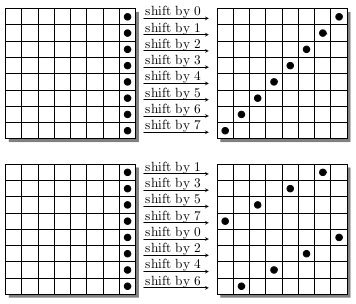
\includegraphics[width=3.6in]{groestl512shift.jpg}
    \end{center}
    \caption{ShiftBytes transformation of permutation $P_{512}$(top) and $Q_{512}$(bottom) \cite{00019}}
    \label{fig:lab}
  \end{figure}

  \subsubsection{ShiftBytes:} cyclically shifts the bytes in a row to left by that number. Let list 
  vector of a number denote the shift, with the index of the element indicating the row. The vector representation
  for $P_{512}$ = [0, 1, 2, 3, 4, 5, 6, 7] and $Q_{512}$ = [1, 3, 5, 7, 0, 2, 4, 6]. The shift is shown in figure
  3.4. Those for the larger permutation are $P_{1024}$ = [0, 1, 2, 3, 4, 5, 6, 11]and $Q_{1024}$ = 
  [1, 3, 5, 11, 0, 2, 4, 6]. This shifting is illustrated in figure 3.12 and figure 3.13.
    
  \begin{figure}
    \begin{center}
      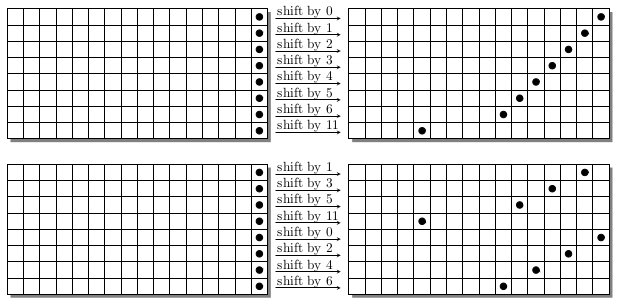
\includegraphics[width=6.4in]{groestl1024shift.jpg}
    \end{center}
    \caption{ShiftBytes transformation of permutation $P_{1024}$(top) and $Q_{1024}$(bottom) \cite{00019}}
    \label{fig:lab}
  \end{figure}

  \begin{center}
  $\mathsf{B} = \renewcommand\arraystretch{0.75}
  \begin{bmatrix}
  \mathsf{02} & \mathsf{02} & \mathsf{03} & \mathsf{04} & \mathsf{05} & \mathsf{03} & \mathsf{05} & \mathsf{07} \\
  \mathsf{07} & \mathsf{02} & \mathsf{02} & \mathsf{03} & \mathsf{04} & \mathsf{05} & \mathsf{03} & \mathsf{05} \\
  \mathsf{05} & \mathsf{07} & \mathsf{02} & \mathsf{02} & \mathsf{03} & \mathsf{04} & \mathsf{05} & \mathsf{03} \\
  \mathsf{03} & \mathsf{05} & \mathsf{07} & \mathsf{02} & \mathsf{02} & \mathsf{03} & \mathsf{04} & \mathsf{05} \\
  \mathsf{05} & \mathsf{03} & \mathsf{05} & \mathsf{07} & \mathsf{02} & \mathsf{02} & \mathsf{03} & \mathsf{04} \\
  \mathsf{04} & \mathsf{05} & \mathsf{03} & \mathsf{05} & \mathsf{07} & \mathsf{02} & \mathsf{02} & \mathsf{03} \\
  \mathsf{03} & \mathsf{04} & \mathsf{05} & \mathsf{03} & \mathsf{05} & \mathsf{07} & \mathsf{02} & \mathsf{02} \\
  \mathsf{02} & \mathsf{03} & \mathsf{04} & \mathsf{05} & \mathsf{03} & \mathsf{05} & \mathsf{07} & \mathsf{02} \\
  \end{bmatrix}$
  \end{center}
  
  \subsubsection{MixBytes:} multiplies each column of the state matrix A, by a constant 8 $\times$ 8 matrix B.
  The transformation, can be shown as $ A \gets B \times A$. The matrix B, can be seen as a finite field over 
  $\mathbb{F}_{256}$, which is shown above. The finite field is defined over 
  $\mathbb{F}_{2}$ by the irreducible polynomial $x^{8} \oplus x^{4} \oplus x^{3} \oplus x \oplus 1$.
  % The composition of matrix B is shown, in appendix A, in item 2.
  %The bytes of the state matrix are in $\mathbb{F}_{256}$ in polynomials of degree at most 7, and coefficients in 0 and 1.
  %The matrix B, is circular shifting of the same row. Each row of the matrix below the current row, is rotated left by
  %a place.
